\section{Reference Time Cuts} \label{sec:reftime}

Fig~\ref{fig:reference_time_cartoon} illustrates the relationship
between a detector signal and the internal clocks of the CAEN 1190 TDCs that
determine the timing resolution of measurements in Hall C.
An L1 pretrigger (see Section~\ref{sec:daq}) that initiates read-out
in a ROC latches onto the leading edge of the next cycle of an 1190's
\SI{40}{\mega\hertz} clock.
As a result, this digitized pretrigger time can only be known to have been
received within the \SI{25}{\nano\second} window between that
\SI{40}{\mega\hertz} cycle and the previous cycle.
Pretriggers also have an intrinsic \SI{4}{\nano\second}
jitter\footnote{A small, irregular variation in an otherwise periodic signal.},
meaning that raw TDC signals can only be known to within
\SI{\sim29}{\nano\second}.
To improve the timing resolution, the DAQ sends a delayed copy of the
pretrigger, called a \textit{reference time}, to a TDC.
The reference time latches onto the leading edge of the 1190's
\SI{10}{\giga\hertz} clock (accurate to \SI{0.1}{\nano\second}), and initiates
read-out of the full TDC spectrum (a lookback window of a few
\si{\micro\second}).
All modules in a given ROC share the same reference time.
Therefore, subtracting the raw TDC time (synced to the \SI{40}{\mega\hertz}
clock) from the reference time (synced to the \SI{10}{\giga\hertz} clock),
the timing resolution can be improved to approximately \SI{0.1}{\nano\second}.
This reference time subtraction is performed offline during hcana
replay.


\begin{figure}[!h]
    \centering
    \includegraphics[width=1.0\textwidth]{chap4/yero_reftime.pdf}
    \caption[Scheme illustrating the synchronization of a detector signal
            with a CAEN 1190 TDC's internal \SI{4}{\mega\hertz} and
            \SI{10}{\giga\hertz} clocks.]{
            Scheme illustrating the synchronization of a detector signal
            with a CAEN 1190 TDC's internal \SI{4}{\mega\hertz} and
            \SI{10}{\giga\hertz} clocks. Figure reproduced from Carlos Yero's
            PhD thesis~\cite{Yero_2020}.
            }
    \label{fig:reference_time_cartoon}
\end{figure}


As shown in Fig~\ref{fig:raw_tdc_time},
true physics events will lie within a range of approximately 300 raw TDC
channels.
Background events will have occurred earlier in the lookback window, and must
be prevented from being chosen as the reference time.
To accomplish this, hcana uses reference time cuts defined in
the parameter files.
Any hits outside the minimum and maximum TDC range will be ignored.

\begin{figure}[!h]
    \centering
    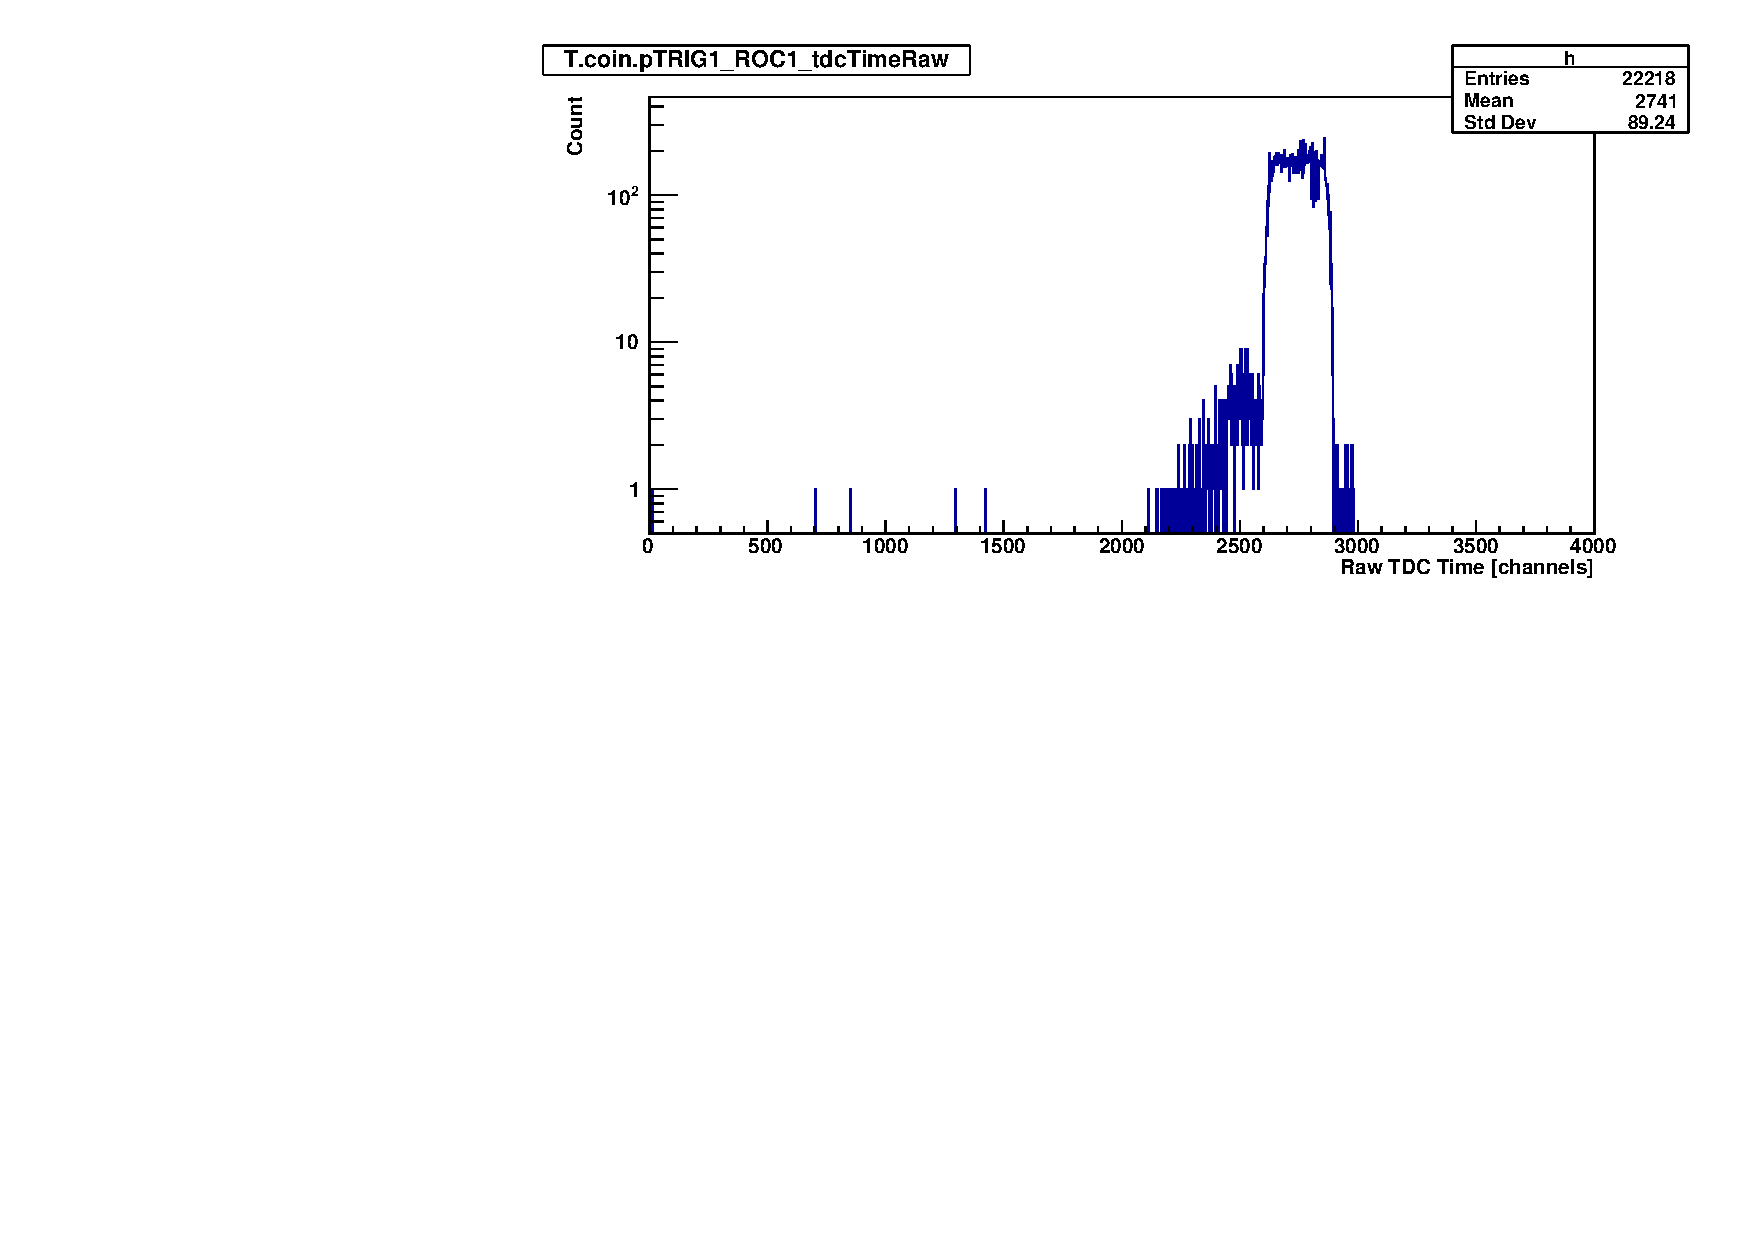
\includegraphics[width=1.0\textwidth]{chap4/coin3192_T_coin_pTRIG1_ROC1_tdcTimeRaw.pdf}
    \caption[
            The raw TDC time spectrum in channels for the trigger formed by
            coincidence of three of four hodoscope planes in the SHMS.]{
            The raw TDC time spectrum in channels for the trigger formed by
            coincidence of three of four hodoscope planes in the SHMS.
            True physics events lie in the plateau from approximately
            2600 to 2900 channels.
            Hits outside this plateau are background that will be ignored by
            hcana if the minimum and maximum cuts are set tightly around the
            plateau.
            }
    \label{fig:raw_tdc_time}
\end{figure}

\section{Detector Time Window Cuts}
As with reference time selection, care must be taken to avoid background hits
in the fADC spectra.
The distribution of the differences between the fADC pulse times and
reference-time-subtracted TDC times for a given PMT in a detector should
be a narrow peak with a width determined by the resolutions of the TDCs
and fADCs.
Events far from this peak have TDC and fADC times that are not correlated, and
can be assumed not to be associated with the current event.
By placing lower and upper bounds on the difference between these times on a
per-PMT basis, we can ensure that hcana will choose the correct fADC
hits for every event.
Representative histograms of these time differences are shown in
Fig~\ref{fig:cal_goodNegAdcTdcDiffTime}.


\begin{figure}[!h]
    \centering
    \includegraphics[width=1.0\textwidth]{chap4/plot_scripts/cal_goodNegAdcTdcDiffTime.pdf}
    \caption{
            The difference between fADC pulse times and
            reference-time-subtracted TDC times for six representative PMTs
            on one side of one plane of the HMS calorimeter.
            }
    \label{fig:cal_goodNegAdcTdcDiffTime}
\end{figure}
